% vim: set tw=78 tabstop=4 shiftwidth=4 aw ai:

\chapter{Multiparty Protocol in the Linux Kernel}
\label{chapter:multiparty}

The \textit{swift} protocol is a generic multiparty transport protocol. Its
mission is to disseminate content among a swarm of peers. Basically, it
answers one and only one request: \textit{'Here is a hash! Give me data for
it!'}. Such entities as storage, servers and connections are abstracted and
are virtually invisible at the API layer. Given a hash, the data is received
from whatever source available and data integrity is checked cryptographically
with Merkle hash trees.

If you need some data it is somewhat faster and/or cheaper downloading it from
a nearby well-provisioned replica, but on the other hand, this process
requires that multiple parties (e.g. consumers, the data sources, CDN
sites\cite{cdnwiki} , mirrors, peers) have to be coordinate. As the Internet
content  is in a continuous increasing nowadays, the overhead of peer/replica
coordination becomes higher then the mass of the download itself. Thus, the
niche for multiparty transfers expands. Still, current, relevant technologies
are tightly coupled to a single use case or even infrastructure of a
particular corporation. These are the reasons of the \textit{swift} protocol
appearance with its primary goal to act as a generic content-centric
multiparty transport protocol that allows seamless, effortless data
dissemination on the big cloud represented by the Internet.

\section{Swift Description}
\label{sec:multiparty:description}

Most features of the \textit{swift} protocol are defined by its function as a
content-centric multiparty transport protocol. A significant difference
between \textit{swift} and the TCP protocol is that TCP possesses no
information regarding what data it is dealing with, as the data is passed from
the user-space, while the \textit{swift} protocol has data fixed in advance
and many peers participate in distributing the same data. Because of this and
the fact that for \textit{swift} the order of delivery is of little importance
and unreliability is naturally compensated for by redundancy, it entirely
drops TCP's abstraction of sequential reliable data stream delivery. For
example, out-of-order data could still be saved and the same piece of data
might always be received from another peer.

Being implemented over UDP, the protocol does its best to make every datagram
self-contained so each datagram could be processed separately and a loss of
one datagram must not disrupt the flow. Thus, a datagram carries zero or more
messages, and neither messages nor message interdependencies should span over
multiple datagrams.

The verification of data pieces is realize using Merkle hash
trees\cite{merkle}, \cite{merkle-ext}. That means that all hashes necessary
for verifying data integrity needs to be put into the same datagram as the
data. For both use cases, streaming and downloading, an unified  integrity
checking scheme that works down to the level of a single datagram is
developed. As a general rule, the sender should append to the data some
meta-data represented by the necessary hashes for the data verification. While
some optimistic optimizations are definitely possible, the receiver should
drop data if it is impossible to verify it. Before sending a packet of data to
the receiver, the sender inspects the receiver's previous acknowledgments to
derive which hashes the receiver already has for sure.

The data is acknowledged in terms of binary intervals, with the base interval
of 1KB "packet". As a result, every single packet is acknowledged logarithmic
number of times. This mechanism provides some necessary redundancy of the
acknowledgements and sufficiently compensates the unreliability of the
datagrams.

The only function of TCP that is also critical for \textit{swift} is the
congestion control. To facilitate delay-based congestion control an
acknowledgment contains besides the dimension of the file received from its
addressee a timestamp.

Our main objective is to integrate \textit{swift} as a transport protocol in
the Linux kernel networking stack. This will provide notable performance
improvement regarding data transfer. We intend to do this with minimal
intrusion effect in the Linux kernel and also to change as little as possible
the current \textit{swift} implementation. Another goal is to provide a
transparent API between the kernel and the user space. A developer will use a
socket-like interface when building an application on top of the
\textit{swift} protocol. In order to achieve this goal we have implemented an
intermediary step. We have simulated the kernel part in the user-space using
raw sockets. This has the advantage of providing means to have modular
functionality tests.

\section{Preliminary Work}
\label{subsec:multiparty:preliminary-work}

While designing our system, we have tackled a few different ideas, each with
its strengths and weaknesees. We present now some of those preliminary ideas
that lead to the our current desing choice.

The first approach we thought of was to include all of the swift protocol into
the kernel space. This approach had the advantage of simplicity and would have
implied minimal architectural changes. The current user space implementation
could have been ported to a kernel module.

Though simple, this approach could not be implemented because of the
restriction of memory size in the kernel.  For the integrity check the swift
protocol relies on Merkle hash tree. Keeping this tree in the kernel space
memory is not scalable. The Internet content is too large to be stored in
kernel. Even if the tree retains only hashes of the data disseminated, the
space is insufficient.

\begin{figure}
  \centering
  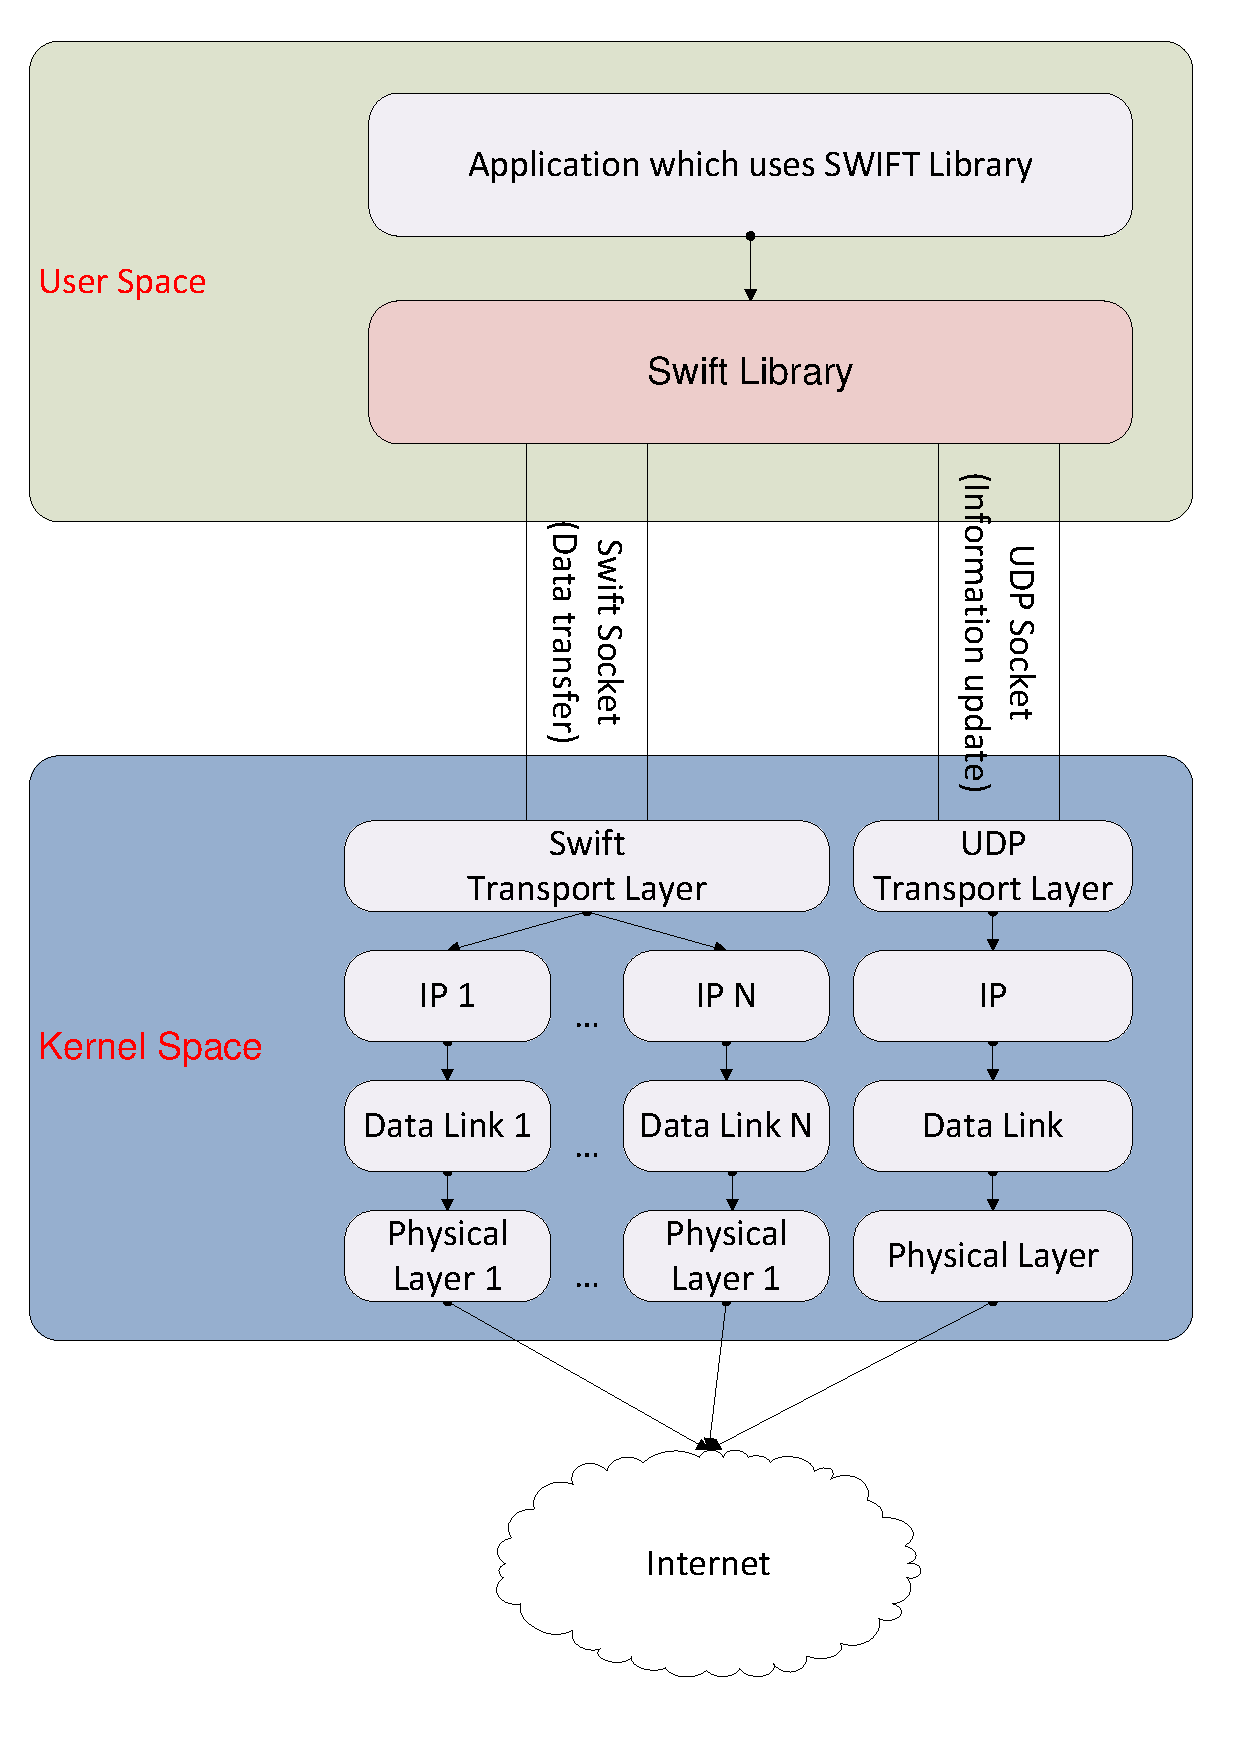
\includegraphics[width=0.4\textwidth]{src/img/multiparty/preliminary-architecture}
  \caption{Preliminary Architecture}
  \label{fig:multiparty:preliminary-architecture}
\end{figure}

The second approach of the swift implementation is represented in the
Figure~\ref{fig:multiparty:preliminary-architecture}. The swift transport
should have been a new kernel interface allowing the creation of specialized
swift sockets. It should have implemented the multiparty protocol allowing
piece transport to/from other hosts in a peer-to-peer fashion.

That implementation should have had specialized "request queues", metadata
queues, to/from user space. Specialized system call API should have allowed
user space applications to interact with the above mentioned queues and, thus,
with the multiparty transport protocol implementation.

Innate differences from a classical one-to-one communication such as UDP or
TCP means the system call API shouldn't have followed the classical
send/receive paradigm. In order to compensate this and to provide a rather
"friendly" interface to user space applications, a library was designed that
to provide a simpler interface. Peer and piece discovery should have been the
responsibility of the user space application. The SWIFT Library may also
provide wrappers over a UDP-based channel for discovery.

Merkle hashes should have stored and computed in user space. This approach
couldn't be implemented because of the restriction of the library
implementations (e.g. a users application design would be more restrictive).
Moreover the kernel implementation should have been like an UDP which support
multicast transfer.

The third approach of the swift implementation was to detach the transport
layer from the original swift implementation and to manage it. When we started
to implement this we found a lot of inconvenience like our code duplicate a
lot of application code, we cannot implement the discovery protocol, and again
our kernel implementation should have been like a multicast-UDP.

This approach also couldn't be implemented because of the complexity of the
transport layer management, moreover we didn't find strengths to confirm that
our implementation could be better than original implementation.

\section{Architecture}
\label{sec:multiparty:architecture}

In this section we present our current architectural design along with the
motivation of choices. We are also going to detail our protocol and the packet
structure used.

In figure Figure~\ref{fig:multiparty:architecture-overview} we see the main
conceptual modules: Application module, wrapper library, peer discovery
overlay and the swift transport protocol layer.

\begin{figure}
  \centering
  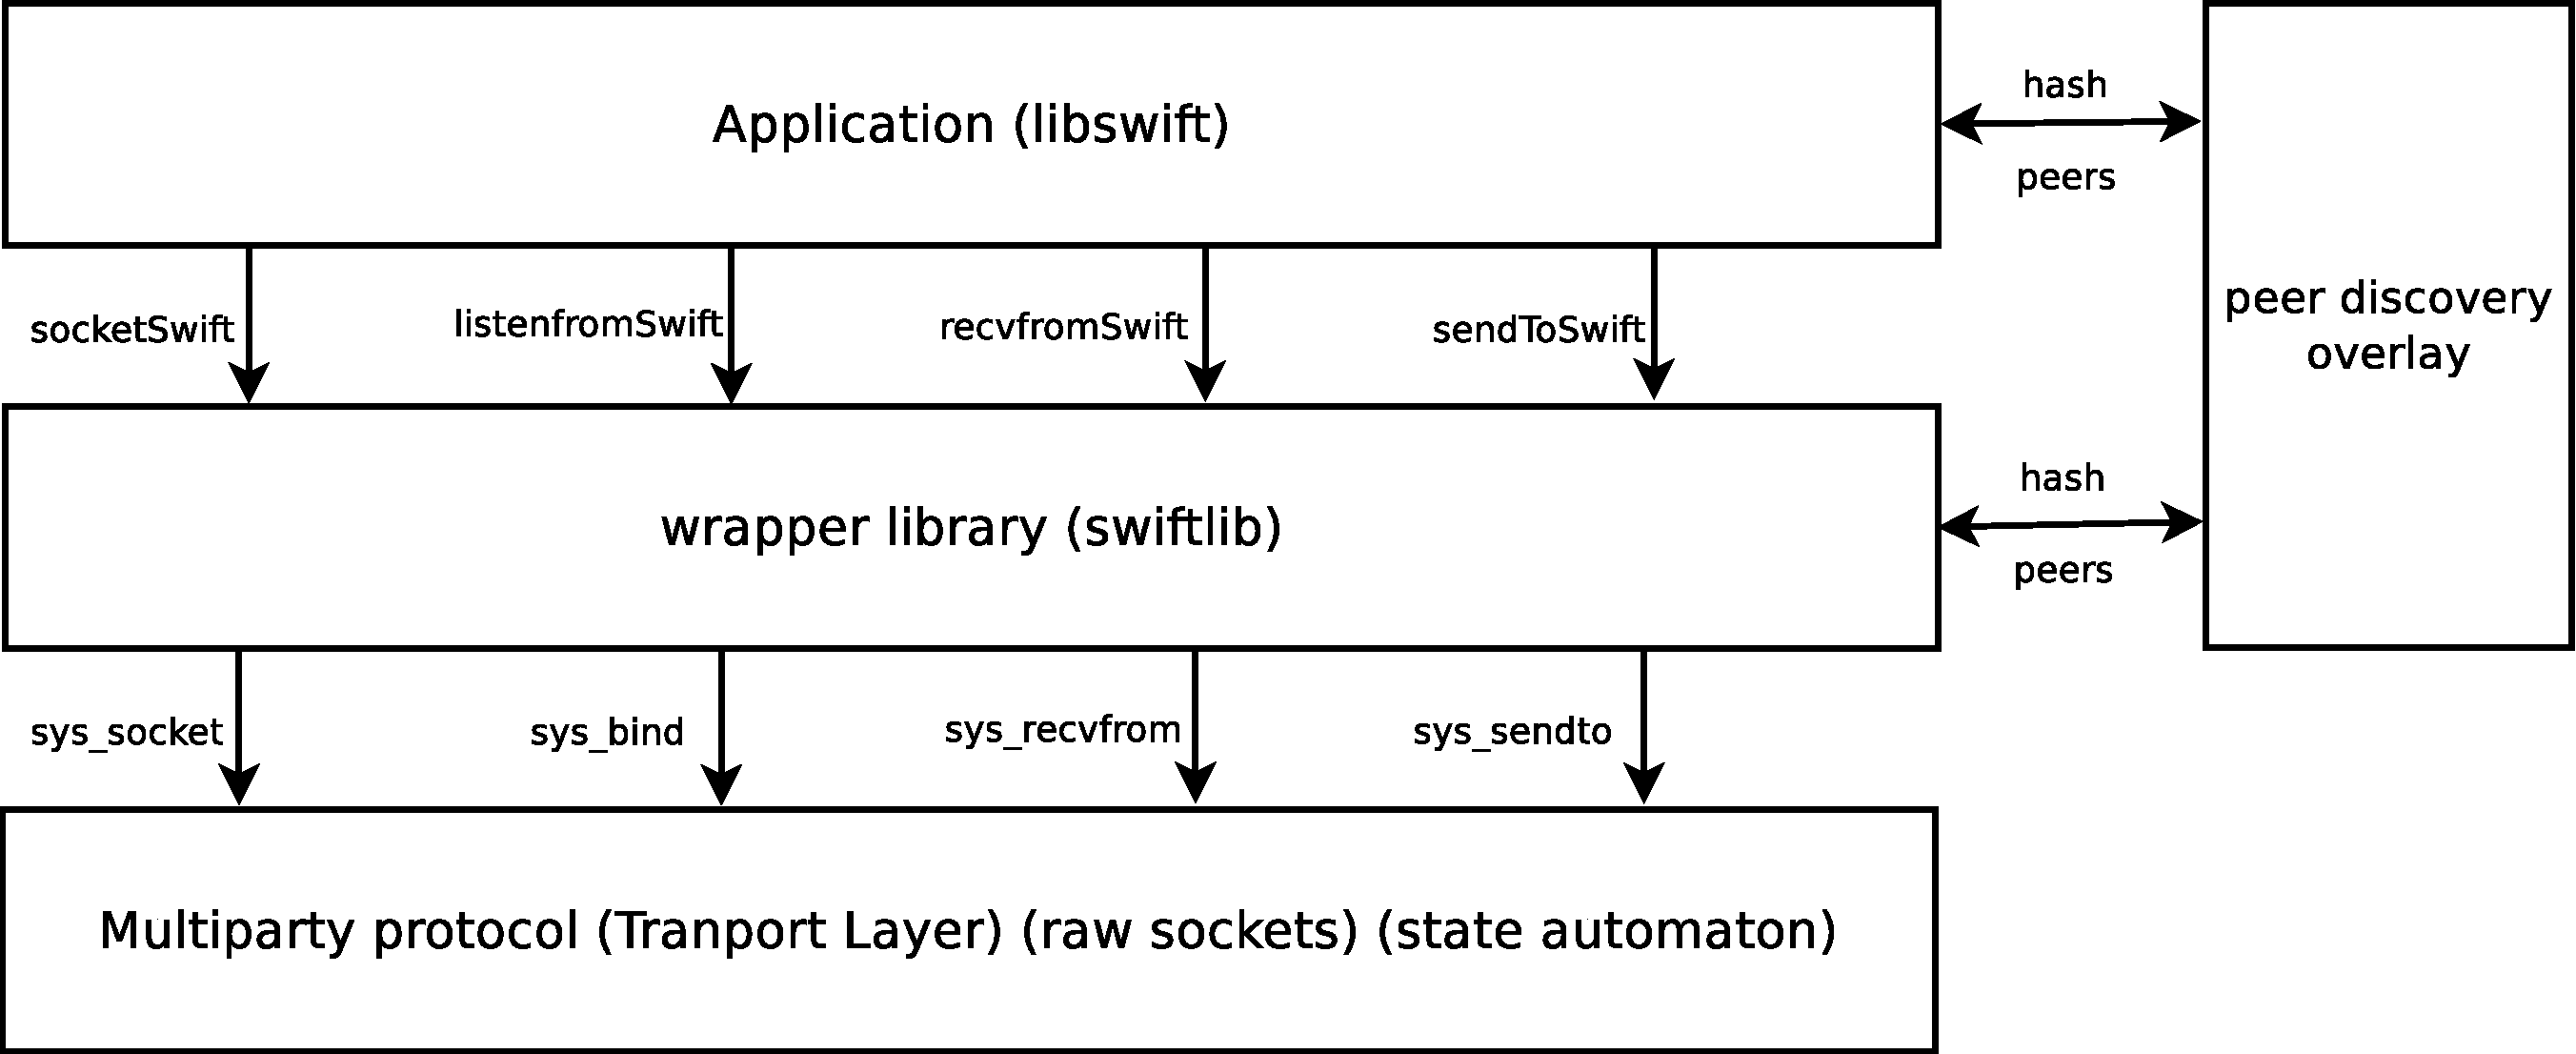
\includegraphics[width=0.4\textwidth]{src/img/multiparty/architecture-overview}
  \caption{Overview Architecture}
  \label{fig:multiparty:architecture-overview}
\end{figure}

The Application module represents the remaining part of the old swift
implementation. This is the part that remains in user space and contains the
file management and hash management features. 

The wrapper library module defines a socket-like API for the user space
applications. An regular program will use those calls instead of the normal
socket ones to use the multiparty sockets. For the moment those calls are
simulated system calls that initially are resolved with the socket raw
implementation (still in user space). In the future this wrapper library
will represent entry points into the kernel.

The peer discovery overlay will remain unchanged. It is still going to work
based on UDP sockets and link the same levels in the swift implementation as
before. The peer discover will be part of the application implementation and
it will be at the developer choice how to implement and how to manage it.

The multiparty protocol is implemented for now at user space level by a raw
socket layer to validate our architecture.  This has the advantage of
simulating the real design modularization but also permit an easier debugging
and testing procedure of the integration. In the next step this part will be
represented by a kernel patch that will communicate through custom made system
calls with the wrapper library. This two phases are described in
Figure~\ref{fig:multiparty:detailed-architecture}.

\begin{figure}
  \centering
  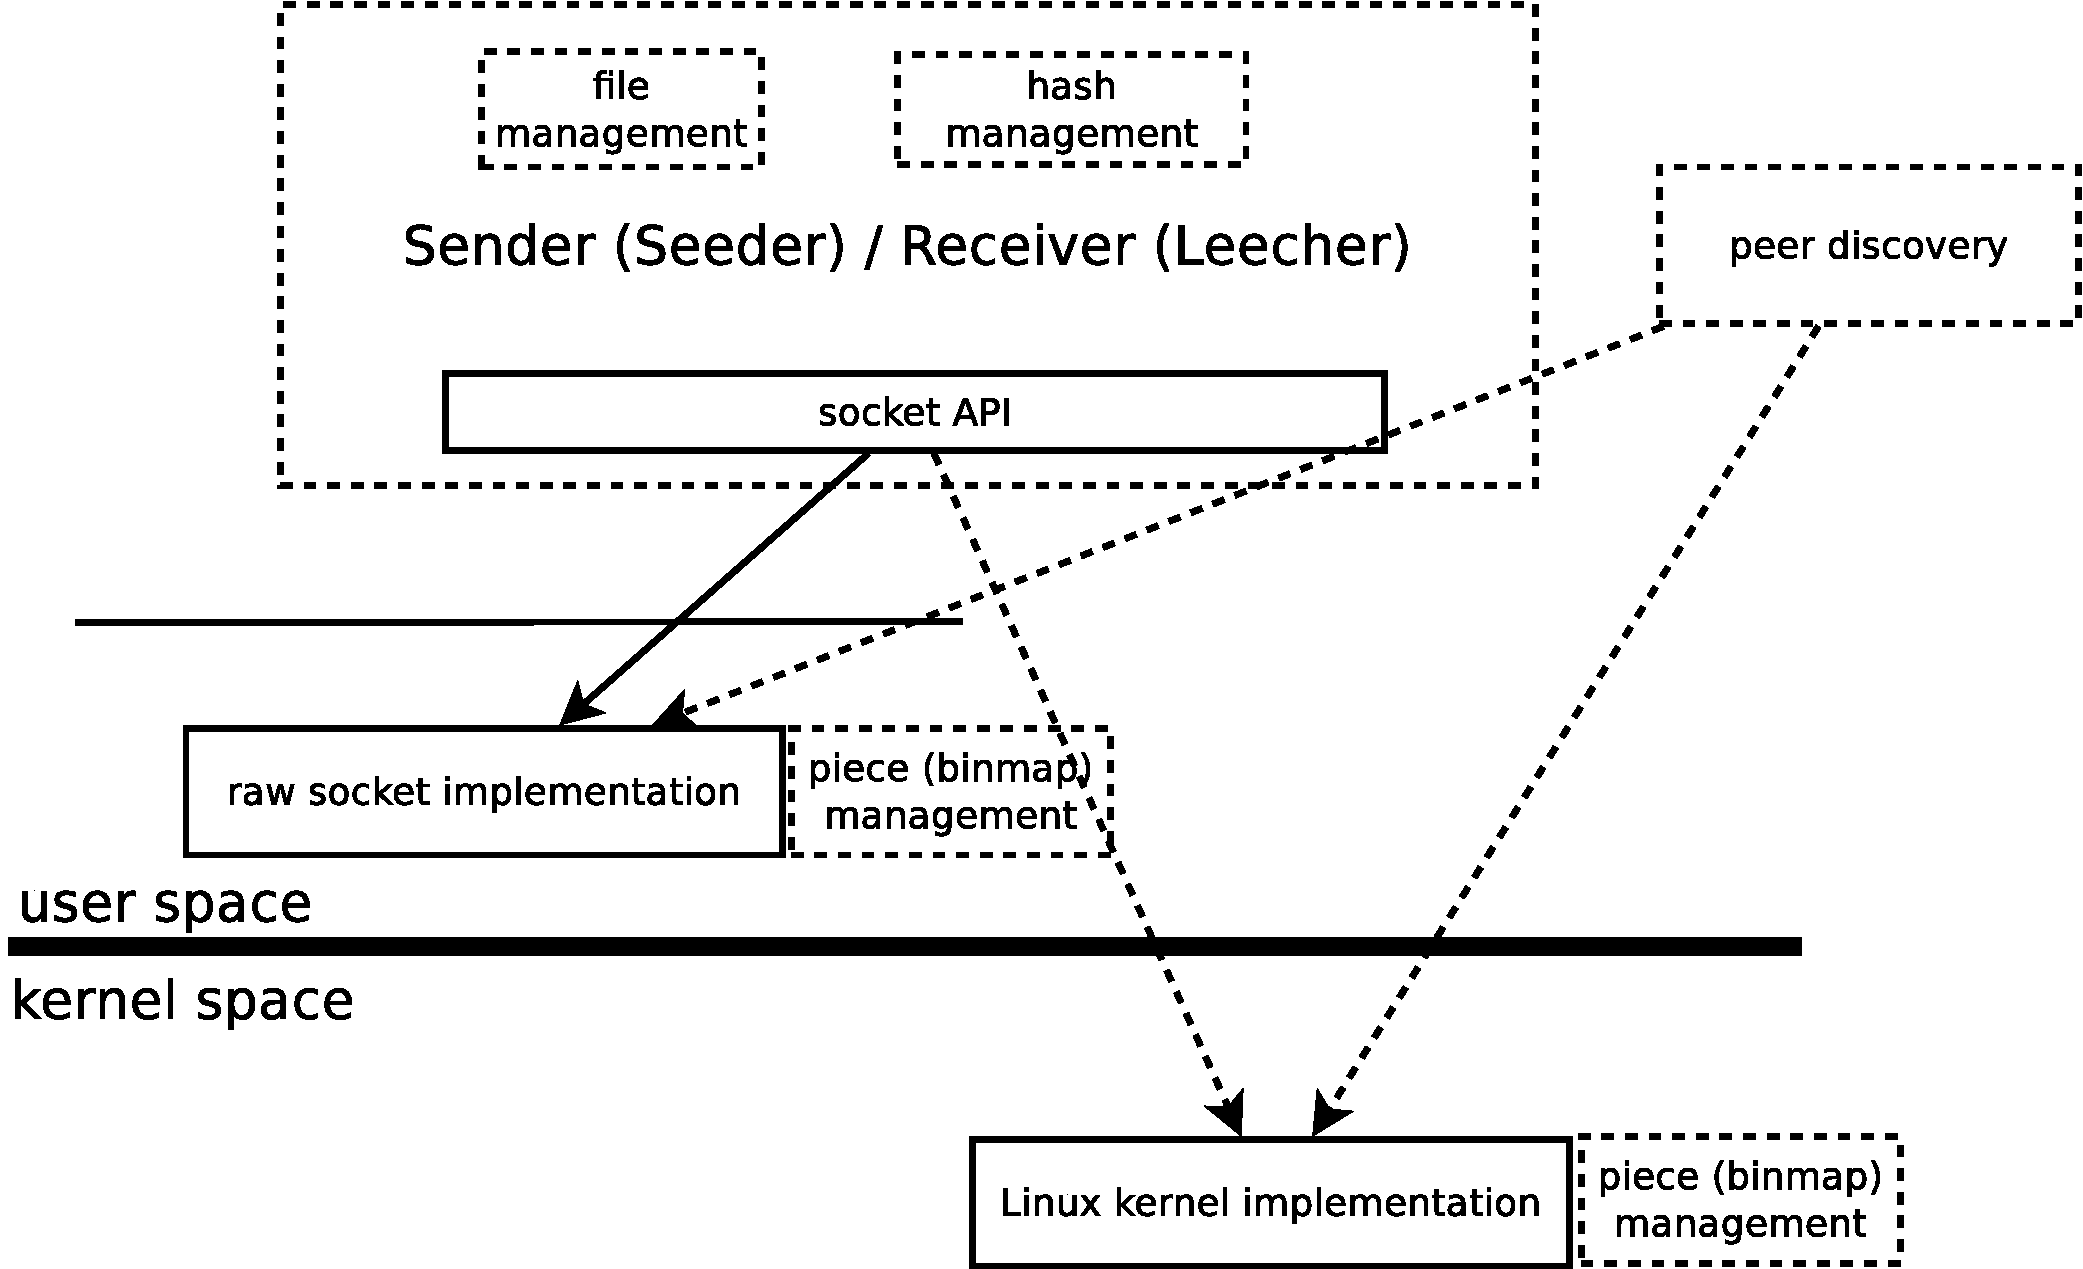
\includegraphics[width=0.4\textwidth]{src/img/multiparty/detailed-architecture}
  \caption{Detailed Architecture}
  \label{fig:multiparty:detailed-architecture}
\end{figure}

A socket is one of the most fundamental technologies of computer networking.
Sockets allow applications to communicate using standard mechanisms built into
network hardware and operating systems.

Raw mode is basically there to allow you to bypass some of the way that your
computer handles TCP/IP. Rather than going through the normal layers of
encapsulation/decapsulation that the TCP/IP stack on the kernel does, you just
pass the packet to the application that needs it. No TCP/IP processing -- so
it's not a processed packet, it's a raw packet. The application that's using
the packet is now responsible for stripping off the headers, analyzing the
packet, all the stuff that the TCP/IP stack in the kernel normally does for
you.

Raw socket implementation will support all syscalls and it will be a copy of
our kernel implementation.  This implementation will have the same API and
behavior as the kernel implementation. Still, in the first implementation, a
swift socket will be available to act as only a seeder or a leecher,
explicitly one operation transmit data or receive data will be supported.

In the last implementation the swift protocol will be develop in kernel space,
and it will be accessible with a datagram socket that will support all socket
syscalls. It will intend to support both operations (receive / send) data over
only one socket.

\begin{figure}
  \centering
  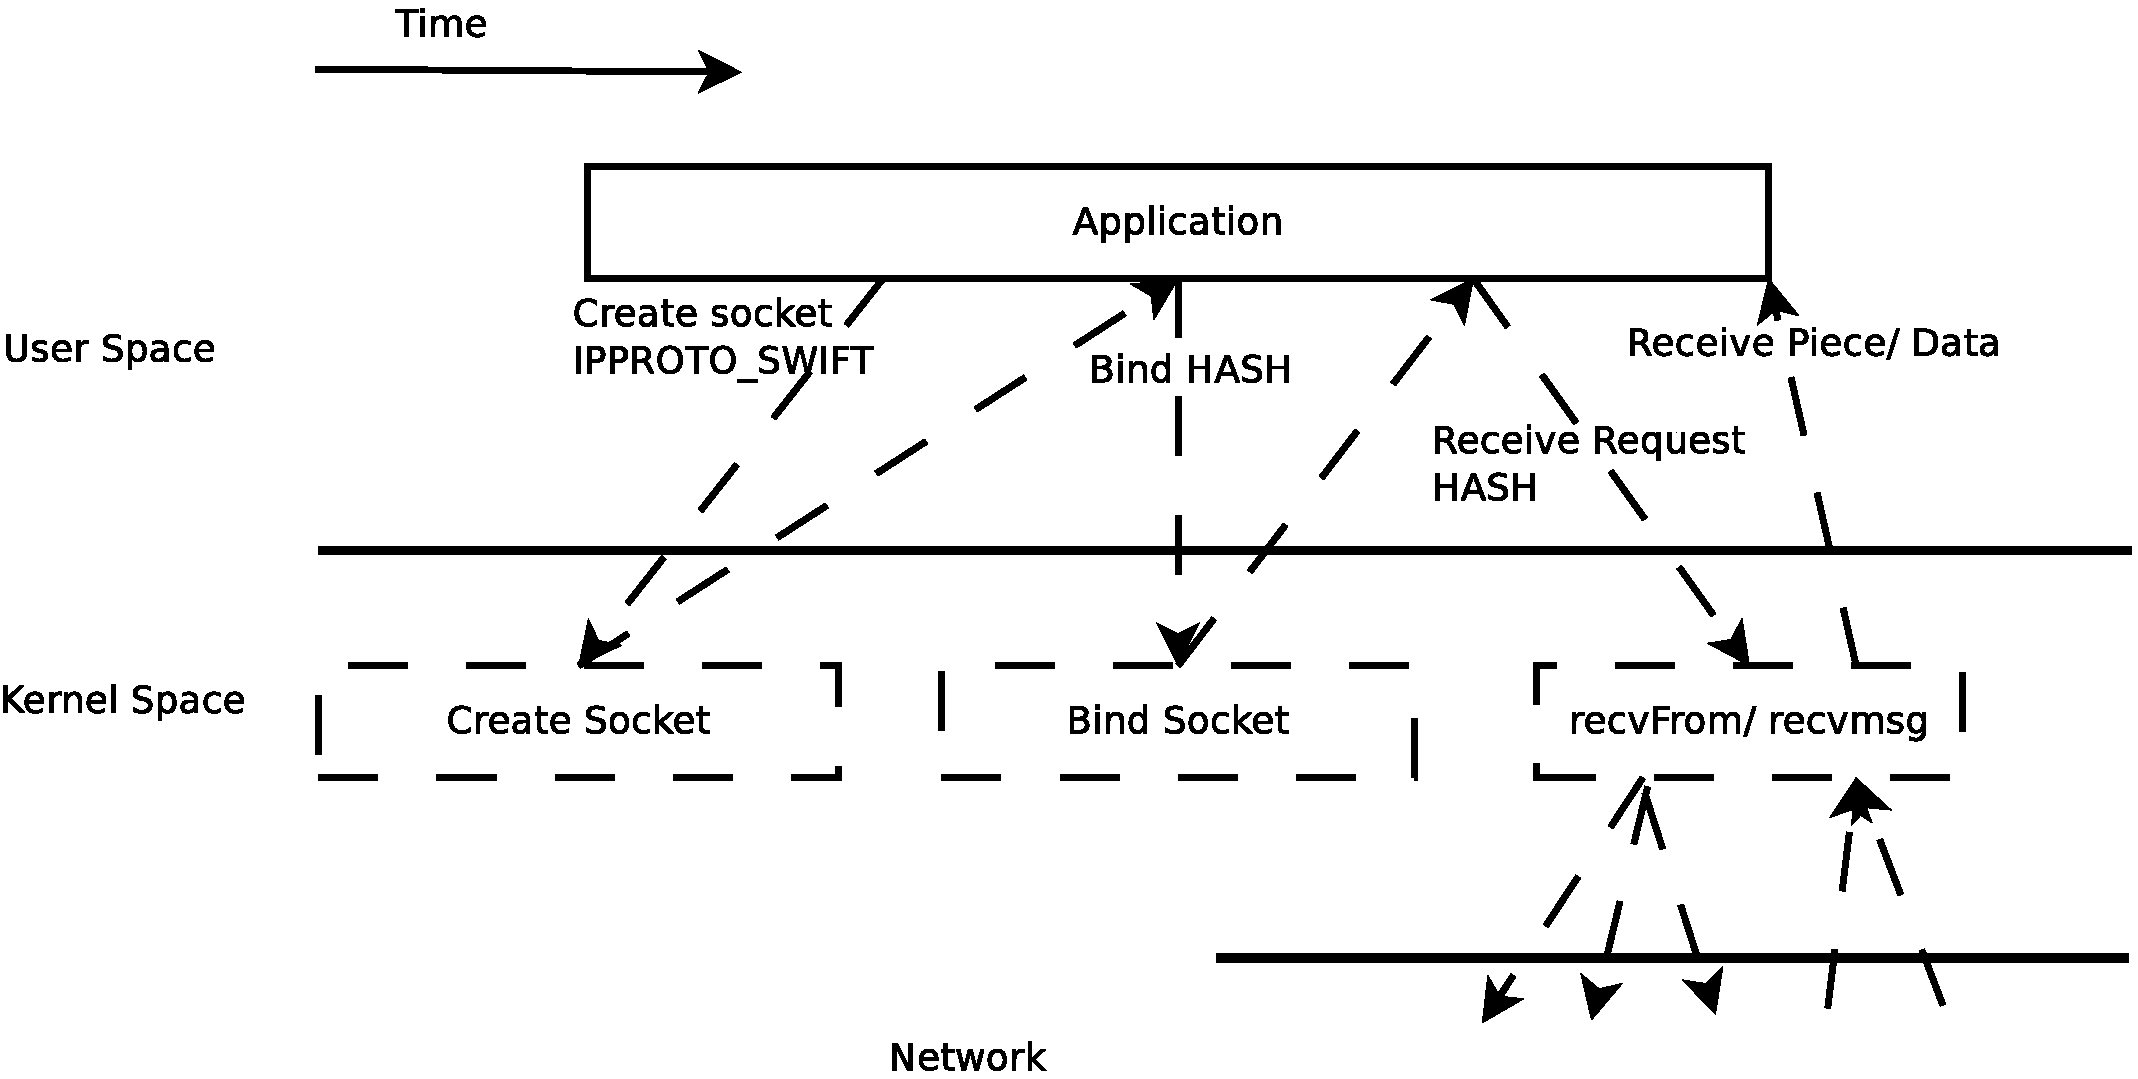
\includegraphics[width=0.55\textwidth]{src/img/multiparty/multiparty-recvmsg}
  \caption{Leecher Conceptual Model}
  \label{fig:multiparty:multiparty-recvmsg}
\end{figure}

Figure~\ref{fig:multiparty:multiparty-recvmsg} presents the conceptual model
of the Leecher. The Leecher is the one that wants to receive a data. In order
to do this it must connect to the multiparty protocol by creating and binding
to a multiparty socket. When it binds to a socket, it uses the hash as a
parameter to find a connection with a peer that has the respective file. This
discovery is done the peer discovery overlay. The Leecher then waits for
packets from the seeders.

\begin{figure}
  \centering
  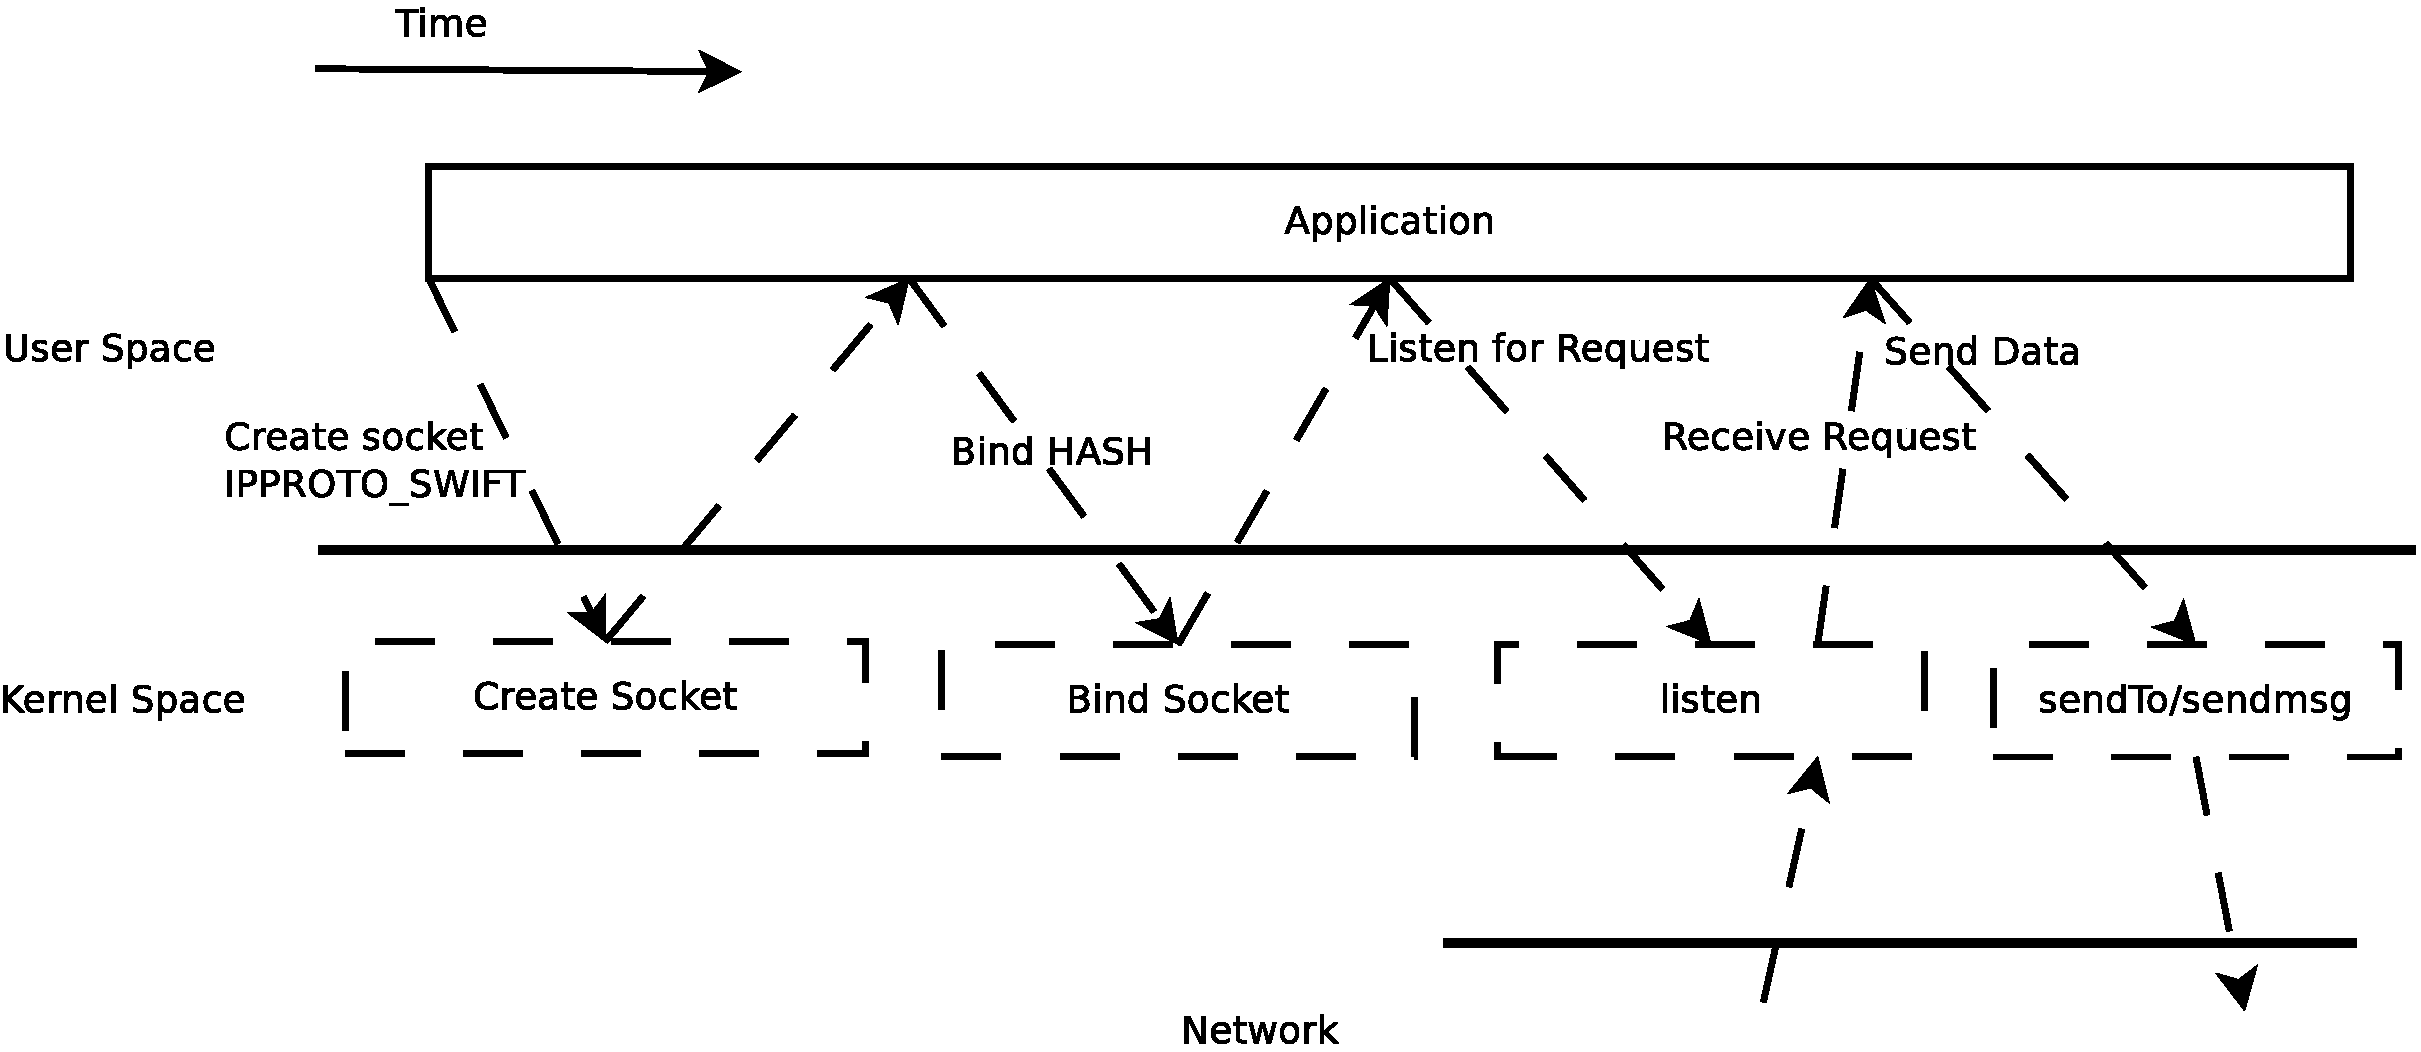
\includegraphics[width=0.55\textwidth]{src/img/multiparty/multiparty-sendmsg}
  \caption{Preliminary Architecture}
  \label{fig:multiparty:multiparty-sendmsg}
\end{figure}

Figure~\ref{fig:multiparty:multiparty-sendmsg} presents the conceptual model
of the Seeder. The Seeder is the one that serves data to other Leechers. In
order to do this it must connect to the multiparty protocol by creating,
binding and listening to a mutliparty socket. When binding the Seeder
practically uses the hash as a parameter. This means that for every file
hashed there will be a socket on which the seeder can receive and serve
requests. The Seeder then waits for requests and sends data packets as
requested.

\section{Testing}
\label{sec:multiparty:testing}

The  protocol is a generic multiparty transport protocol. Its mission is to
disseminate content among a swarm of peers.  Given a hash, the data is
received from whatever source available and data integrity is checked
cryptographically with Merkle hash trees. 

Our main focus when modifying the swift implementation is to have an impact on
time performance. With a communication protocol the greatest latency is
usually generated by waiting for the results from the network. The multiparty
communication model already takes care of this, so the next best thing is to
enhance the application time. We are doing this by decreasing the time
penalties due to context switches between user space and kernel space. The
main idea is to reduce the number of system calls made from user space into
the kernel. This implicitly reduces the number of preemption moments.

Firstly, we have implemented a test suite for every socket system call, which
test all possible cases.  This unit tests are made to ensure the code quality,
and to validate if the system call respond in the same mode as other similar
system call.

Secondly, we have implemented a functional tests to validate a simple
workflow. For this purpose we have a sender that acts as the seeder and a
receiver which have the leecher role. We transfer a small file between this
entities.

Also we will implement performance tests that will validate our design and
implementation. This tests will compare the number of system calls for both
implementation (original implementation and our implementation).

\section{Summary}
\label{sec:multiparty:summary}

The \textit{swift} protocol is a multiparty content-centric protocol that aims
to disseminate content among a swarm of peers. This paper proposes an approach
for the optimization of the currently \textit{swift} protocol. The integration
of the communication in the kernel space as a multiparty transport protocol
that is solely responsible for getting the bits moving improves the over all
protocol performance. It ensures maximum efficiency of data transfer by
decreasing switches between user and kernel space and eliminating some
performance penalties due to context switches.

\subsection{Directions for Future Work}

After we complete the implementation and the functional tests, we want to test
extensively our new features in a real environment. We plan to do stress tests
using a cluster. This tests will help us to make an overview about our
implementation and we could compare with the user-space implementation of the
\textit{swift} to determine exactly what performance we encountered. If the
results are satisfactory, we will continue to optimize our program and we will
add new features.

It will be very useful to have a real application on top of the \textit{swift}
protocol. If not, one solution would be to port an application strictly for
this task. This would give us the opportunity to extend and refine our
implementation, and also to extend the library API.

\section{Kernel-based Implementation of Multiparty Protocol}

Un protocol de transport multiparty este un protocol care suportă participarea
mai multor entități decât în cazul general de client-server.  Unul dintre cele
mai folosite protocoale multiparty este protocolul BitTorrent.

Un fișier care se dorește a fi distribuit prin intermediul protocolului
BitTorrent este împărțit în bucăți, numite pieces. Pe măsură ce aste bucăți
sunt aduse, utilzatorul curent le pune la dispoziție altor utilizatori (el se
transformă din leecher în seeder în momentul în care are tot fișierul pus la
dispoziția celorlalți). Pentru a asigura consistența datelor, fiecare bucată
are asociată un rezumat care se găsește în descriptorul .torrent al
fișierului de download-at.

Unul dintre neajunsurile protocolului BitTorrent a fost faptul că
acesta rulează peste TCP, protocol care asigură primirea pachetelor în
ordine, ceea ce este redundant pentru BitTorrent, deoarece se verifică
oricum consistența datelor la nivel de bucată.

Pentru a rezulva aceasta problemă a fost propus uTP (care este
practic o reimplementare a TCP peste UDP, după parerea unora). Acest
protocol încearcă să rezolve problemele latenței și controlului congestiei
întâlnite în cazul folosirii TCP, în timp ce se asigură consistența primirii
datelor și așezarea bucăților în ordinea corectă. O funcționalitate
importantă a uTP este încetinirea ratei de transfer a pachetelor când
acestea interferează cu alte aplicații, cum ar fi browser-ul de internet.
LEDBAT este un protocol experimental folosit la controlul
congestiei. Scopul lui principal este de a utiliza lațimea de bandă
disponibilă pe un traseu din internet limitând creșterea întârzierii de-a
lungul căii de transport. Protocolul swift se bazează pe LEDBAT pentru
controlul congestiei.

Protocolul swift este implementat in momentul de față în user-
space, folosind socket-i UDP. Nu este nevoie de TCP pentru că siguranța
ordinii oferită de TCP este redundantă în cazul swift. Pachetele pot fi
primite în afara ordinii iar aceeași bucată de date poate fi primită de mai
multe ori, de la peer-i diferiți.

Principala funcționalitate a protoculului swift este că acesta este un
protocol centrat pe tipul conținutului. TCP, de exemplu nu știe ce fel de
date transportă, în timp ce, în cazul swift, are datele fixate suficient de
devreme astfel încât să îi fie cunoscute. De asemenea, mai mulți peer-i
participă la distribuția acelorași date.

Verificarea bucăților primite prin intermediul swift este realizată prin
folosirea unor Merkle hash trees. Asta înseamnă că toate datele necesare
verificării integrității vor fi așezate în același pachet cu datele.

\subsection{Tranport Protocol Implementation on the Linux Kernel}

Pentru a implementa un protocol de transport în nucleul linux
trebuie stabilite următoarele în faza de design:

\begin{itemize}
  \item Definirea \texttt{IPPROTO\_\$\$} care să reprezinte id-ul noului
  protocol de transport. Acesta va fi folosit ulterior la crearea socket-ului.
  \item Definirea header-ului de transport (în framework am definit în header
  două porturi pe 8 biți, unul sursă altul destinație și o lungime pe 16 biți,
  care reprezintă lungimea datelor, incluzând header-ul protocolului de
  transport).
\end{itemize}

După ce aceastea au fost stabilite, trebuie completate următoarele structuri:
\begin{itemize}
  \item O structură în care se definește un socket de tipul nou. Aici trebuie
  să salvăm informații despre starea socketului (de exemplu la ce port
  destinație este conectat sau pe ce port sursă a fost legat).
  \begin{verbatim}
    struct swift_sock {
        struct inet_sock sock;
        /* swift socket speciffic data */
        uint8_t src;
        uint8_t dst;
    };
  \end{verbatim}

  \item O altă structură în care se definește protocolul, prin dimensiunea
  socket-ului și numele acestuia.
  \begin{verbatim}
    static struct proto swift_prot = {
        .obj_size = sizeof(struct swift_sock),
        .owner = THIS_MODULE,
        .name = "SWIFT",
    };
  \end{verbatim}

  \item Cea mai importantă structură este aceea care descrie operațiile care
  sunt suportate de un socket de acest tip.  Pentru un socket prin care se vor
  trimite datagrame, este suficientă implementarea funcțiilor de release,
  bind, connect, sendmsg și recvmsg.
  \begin{verbatim}
    static const struct proto_ops swift_ops = {
        .family = PF_INET,
        .owner = THIS_MODULE,
        .release = swift_release,
        .bind = swift_bind,
        .connect = swift_connect,
        .socketpair = sock_no_socketpair,
        .accept = sock_no_accept,
        .getname = sock_no_getname,
        .poll = datagram_poll,
        .ioctl = sock_no_ioctl,
        .listen = sock_no_listen,
        .shutdown = sock_no_shutdown,
        .setsockopt = sock_no_setsockopt,
        .getsockopt = sock_no_getsockopt,
        .sendmsg = swift_sendmsg,
        .recvmsg = swift_recvmsg,
        .mmap = sock_no_mmap,
        .sendpage = sock_no_sendpage,
    };
    \end{verbatim}

  \item În structura \texttt{net\_protocol} se setează handler-ul pentru
  pachetele de tipul nou create venite de pe țeavă (vor avea setate în câmpul
  protocol din header-ul de IP valoarea noului protocol).
    \begin{verbatim}
    static const struct net_protocol swift_protocol = {
        .handler = swift_rcv,
        .no_policy = 1,
        .netns_ok = 1,
    };
    \end{verbatim}

  \item O ultimă structură care leagă protocul nou creat de structura care
  conține operațiile pe socket-ii acestuia.
    \begin{verbatim}
    static struct inet_protosw swift_protosw = {
        .type = SOCK_DGRAM,
        .protocol = IPPROTO_SWIFT,
        .prot = &swift_prot,
        .ops = &swift_ops,
        .no_check = 0,
    };
    \end{verbatim}
\end{itemize}

În momentul în care avem toate aceste structuri completate, putem adăuga
protocolul în nucleul Linux. Secvența de operații care face acest lucru se
găsește mai jos:

\begin{verbatim}
proto_register(&swift_prot, 1);
inet_add_protocol(&swift_protocol, IPPROTO_SWIFT);
inet_register_protosw(&swift_protosw);
\end{verbatim}

Înainte de a putea compila și insera modului în nucleul Linux, mai trebuie
completate funcțiile pentru socket-i de release, bind, connect, sendmsg și
recvmsg. De asemenea trebuie implementat și handler-ul pentru pachetele venite
din rețea. La nivelul protocolului trebuie ținută o asociere între port și
socket, cu semnificația ca socket-ul este legat de acel port.

În funcția de release se vor elibera resursele ocupate de socket.

În funcția de bind se va verifica portul primit să fie liber, și se va
lega socketul de acest port și de o adresă IP sursă.

Funcția de connect va asocia socket-ul curent cu un port destinație
și cu o adresă IP destinație.

Funcția sendmsg va extrage adresa și portul destinație dacă au fost date ca
parametri la apelul din user-space. Dacă nu au fost date, se verifică dacă
socket-ul este conectat (dacă a existat un apel anterior de connect), iar în
cazul în care nu este nici conectat, se întoarce eroare.  După ce s-a stabilit
către cine se va trimite pachetul și pe ce port, se alocă un skb în care se va
pune header-ul de swift și restul datelor. Se completează header-ul de swift
și se copiaza datele din user-space, după care se face rutarea pachetului
(trebuie să aflăm pe ce adresă IP sursă va ieși pachetul). După rutare, se
copiaza informațiile necesare în socket și se pune în coada de trimitere
pachetul folosind \texttt{ip\_queue\_xmit}.

Funcția recvmsg face operația inversă funcției de sendmsg. Se citește o
datagramă din coada de primire folosind \textbf{skb\_recv\_datagram} se fac
unele verificări de consistență a datelor, după care se copiază informațiile
din skb în user-space. De asemenea, în situația în care a fost cerută și
adresa de la care a venit pachetul (la apelul recvmsg sau recvfrom), se
completează aceste informații. La sfârșit se eliberează structura skb folosind
\texttt{skb\_free\_datagram}.

Funcția trecută în handler în structura \texttt{net\_protocol}, va fi apelată la
primirea din rețea a unui pachet de tipul protocolului curent. În momentul
primirii pachetului, se face diverse validari ale acestuia, după care se
extrage portul destinație. Se caută socket-ul pentru acest port destinație
în maparea din interiorul protocolului, se salvează în skb->cb informații
despre cel care a generat pachetul după care se pune pachetul în coada
pentru receive folosind \texttt{ip\_queue\_rcv\_skb}.

\subsection{Testing}

Testarea protocolului se va face prin intermediul unor unit teste.
Printre acestea se găsesc câteva teste simple, pentru asigurarea
funcționalității de bază, la care se adaugă teste care verifică situațiile de
eroare și teste care verifică performanța protocolului (asigurarea
scalabilității – mai mulți clienți în același timp).

Testarea funcționalităților de bază se va face pentru fiecare funcție
expusă de protocol (se vor face teste pentru bind, connect, close,
sendto, recvfrom, sendmsg, recvmsg, send și recv).

Testarea negativă, pentru situații limită se va face la fel, pentru fiecare
funcție expusă de modul. În cazul funcției de bind se va verifica întoarcerea
erorii în cazul apelulului duplicat folosind același port. La fel se va face
și pentru folosirea de adrese, porturi invalide. Câte o serie de astfel de
teste se va face pentru fiecare funcționalitate.

Testarea performanței se va face folosind mai mulți socket-i,
verificând dacă datele trimise pe un socket ajung pe socket-ul destinație
corespunzător (practic se verifică dacă maparea între porturi și socket-i
funcționeaza corespunzător). O altă măsură a performanței este viteza de
transfer folosind socket-ul nou creat.

\subsection{Conclusion and Future Work}

Swift este un protocol multiparty prin care se va distribui conținut între
peer-ii din Internet. Acest protocol poate fi adus la nivelul nucleulului
Linux prin adaptarea acestuia la framework-ul descris în acest document. Prin
aducerea protocolului la nivelul nucleului performanța ar trebui să fie
îmbunătățită deoarece numărul de schimbări de context între user-mode și
kernel-mode se va micșora considerabil (numărul de apeluri de sistem va
scădea).

Framework-ului îi lipsește în momentul de față un mecanism de fragmentare a
datelor în pachete mai mici. Practic, cu implementarea de față, nu se poate
trimite pe un socket un volum de date util mai mare decât MTU (1500) –
sizeof(iphdr) – sizeof(swifthdr). O soluția ar fi împrumutarea mecanismului de
framgmentare de la implementarea UDP.
